%%% Hlavní soubor. Zde se definují základní parametry a odkazuje se na ostatní části. %%%

%% Verze pro jednostranný tisk:
% Okraje: levý 40mm, pravý 25mm, horní a dolní 25mm
% (ale pozor, LaTeX si sám přidává 1in)
\documentclass[12pt,a4paper]{report}
\setlength\textwidth{145mm}
\setlength\textheight{247mm}
\setlength\oddsidemargin{15mm}
\setlength\evensidemargin{15mm}
\setlength\topmargin{0mm}
\setlength\headsep{0mm}
\setlength\headheight{0mm}
% \openright zařídí, aby následující text začínal na pravé straně knihy
\let\openright=\clearpage

%% Pokud tiskneme oboustranně:
% \documentclass[12pt,a4paper,twoside,openright]{report}
% \setlength\textwidth{145mm}
% \setlength\textheight{247mm}
% \setlength\oddsidemargin{14.2mm}
% \setlength\evensidemargin{0mm}
% \setlength\topmargin{0mm}
% \setlength\headsep{0mm}
% \setlength\headheight{0mm}
% \let\openright=\cleardoublepage

%% Vytváříme PDF/A-2u
\usepackage[a-2u]{pdfx}

%% Přepneme na českou sazbu a fonty Latin Modern
%\usepackage[czech]{babel}
\usepackage{lmodern}
\usepackage[T1]{fontenc}
\usepackage{textcomp}

%% Použité kódování znaků: obvykle latin2, cp1250 nebo utf8:
\usepackage[utf8]{inputenc}

%%% Další užitečné balíčky (jsou součástí běžných distribucí LaTeXu)
\usepackage{amsmath}        % rozšíření pro sazbu matematiky
\usepackage{amsfonts}       % matematické fonty
\usepackage{amsthm}         % sazba vět, definic apod.
\usepackage{bbding}         % balíček s nejrůznějšími symboly
			    % (čtverečky, hvězdičky, tužtičky, nůžtičky, ...)
\usepackage{bm}             % tučné symboly (příkaz \bm)
\usepackage{graphicx}       % vkládání obrázků
\usepackage{fancyvrb}       % vylepšené prostředí pro strojové písmo
\usepackage{indentfirst}    % zavede odsazení 1. odstavce kapitoly
\usepackage{natbib}         % zajištuje možnost odkazovat na literaturu
			    % stylem AUTOR (ROK), resp. AUTOR [ČÍSLO]
\usepackage[nottoc]{tocbibind} % zajistí přidání seznamu literatury,
                            % obrázků a tabulek do obsahu
\usepackage{icomma}         % inteligetní čárka v matematickém módu
\usepackage{dcolumn}        % lepší zarovnání sloupců v tabulkách
\usepackage{booktabs}       % lepší vodorovné linky v tabulkách
\usepackage{paralist}       % lepší enumerate a itemize
\usepackage{xcolor}         % barevná sazba

\usepackage{rotating}
%\usepackage{fontspec}
\usepackage{tipa}
\usepackage{enumitem}
\usepackage{makecell}
\usepackage{alltt}
\usepackage{refcount}
\usepackage{tabularx}
\usepackage{caption}


%%% Údaje o práci

% Název práce v jazyce práce (přesně podle zadání)
\def\NazevPrace{Iterativní zdokonalování přepisu zvukových nahrávek s~využitím zpětné vazby posluchačů}

% Název práce v angličtině
\def\NazevPraceEN{Iterative Improving of Transcribed Speech Recordings Exploiting Listener's Feedback}

% Jméno autora
\def\AutorPrace{Mgr. Jan Oldřich Krůza}

% Rok odevzdání
\def\RokOdevzdani{2020}

% Název katedry nebo ústavu, kde byla práce oficiálně zadána
% (dle Organizační struktury MFF UK, případně plný název pracoviště mimo MFF)
\def\Katedra{Ústav formální a aplikované lingvistiky}
\def\KatedraEN{Institute of Formal and Applied Linguistics}

% Jedná se o katedru (department) nebo o ústav (institute)?
\def\TypPracoviste{Ústav}
\def\TypPracovisteEN{Institute}

% Vedoucí práce: Jméno a příjmení s~tituly
\def\Vedouci{Doc. RNDr. Vladislav Kuboň, Ph.D.}

% Pracoviště vedoucího (opět dle Organizační struktury MFF)
\def\KatedraVedouciho{
  Ústav formální a aplikované lingvistiky\\
  Matematicko-fyzikální fakulta\\
  Univerzita Karlova\\
  Malostranské náměstí 25\\
  11800 Praha 1
}
\def\KatedraVedoucihoEN{Institute of Formal and Applied Linguistics}

% Studijní program a obor
\def\StudijniProgram{informatika}
\def\StudijniObor{matematická lingvistika}

% Nepovinné poděkování (vedoucímu práce, konzultantovi, tomu, kdo
% zapůjčil software, literaturu apod.)

% Abstrakt (doporučený rozsah cca 80-200 slov; nejedná se o zadání práce)
\def\Abstrakt{%
Tato disertační práce se zabývá zpřístupněním zvukových
záznamů jednoho mluvčího úzké i široké veřejnosti.

Motivací práce byla existence chátrajících nahrávek hovorů českého filozofa
ing. Karla Makoně na kazetách a kotoučích. Cílem je zachování materiálu pro
budoucí generace a zpřístupnění nahrávek pomocí digitálních technologií,
především přístupnosti nahrávek na internetu a možnosti vyhledávání v~nich.

Práce představuje tvorbu systému pro přepis velké sady zvukových záznamů
se zapojením laické komunity. Navržené řešení spočívá ve vytvoření základního
přepisu nízké kvality pomocí automatického rozpoznávání řeči a vyvinutí
aplikace, která umožní od členů komunity i nahodilých zájemců získávat opravy
automatického přepisu, použitelné jako trénovací data pro další zlepšování.

Popíše se samotný mluvený korpus. Představí se autor a
jeho dílo,
témata v~nahrávkách, nahrávání samotné, digitalizace a získané přepisy.
Dále se rozvede tvorba systému pro automatický
přepis korpusu od sběru dat, přes akustické a jazykové modelování, různé
provedené experimenty až k~vyhodnocení úspěšnosti. V~neposlední řadě se popíše
webová aplikace pro sběr manuálních přepisů. Zmíní se odlišnosti od ostatních
systémů, detaily návrhu a řešení, mechanismus pro kompenzaci vysokých nároků na kvalitu
přepisu a nízkých nároků na odbornost přispěvatelů a vyhodnocení funkčnosti
po osmi letech provozu.
}
\def\AbstraktEN{%
This Ph.D. thesis deals with making a corpus of audio
recordings of a single speaker accessible to wide public and interested community.

The work has been motivated by the existence of a set of perishing recordings
of the Czech philosopher Karel Makoň on magnetophone tapes. The aim is to conserve
the material for future generations and making it accessible using
digital technologies, in particular publishing the recordings online
and enabling the users to search through them.

The thesis introduces the creation of a system for transcribing a large set of
speech recordings employing a lay community. The solution designed is based on
obtaining a baseline low-quality transcription by means of automated speech
recognition and developing an application that allows for collecting corrections
of the automatic transcription in a fashion that makes it usable as training
data for further improvement of said transcription.

The spoken corpus itself is described. The
author and his works, topics covered in the talks, the process of recording
and digitization as well as the gained transcript are introduced.
Next, the development of a system for automated transcription of
the corpus, from collecting data, to acoustic and language modeling, various experiments
undertaken and evaluation are presented. Then, the web application for gathering
manual transcript corrections is described.
Differences to other settings, design and implementation details, a way to
compensate high demand for transcription quality and low demand for worker
expertise, as well as an evaluation of the system's performance after eight
years of operation are covered.
}

% 3 až 5 klíčových slov (doporučeno), každé uzavřeno ve složených závorkách
\def\KlicovaSlova{%
{přepis zvukových nahrávek} {uživatelská interakce} {komunitní spolupráce}
}
\def\KlicovaSlovaEN{%
{speech transcription} {user inetraction} {community cooperation}
}

%% Balíček hyperref, kterým jdou vyrábět klikací odkazy v PDF,
%% ale hlavně ho používáme k uložení metadat do PDF (včetně obsahu).
%% Většinu nastavítek přednastaví balíček pdfx.
\hypersetup{unicode}
\hypersetup{breaklinks=true}

%% Definice různých užitečných maker (viz popis uvnitř souboru)
%%% Tento soubor obsahuje definice různých užitečných maker a prostředí %%%
%%% Další makra připisujte sem, ať nepřekáží v ostatních souborech.     %%%

%%% Drobné úpravy stylu

% Tato makra přesvědčují mírně ošklivým trikem LaTeX, aby hlavičky kapitol
% sázel příčetněji a nevynechával nad nimi spoustu místa. Směle ignorujte.
\makeatletter
\def\@makechapterhead#1{
  {\parindent \z@ \raggedright \normalfont
   \Huge\bfseries \thechapter. #1
   \par\nobreak
   \vskip 20\p@
}}
\def\@makeschapterhead#1{
  {\parindent \z@ \raggedright \normalfont
   \Huge\bfseries #1
   \par\nobreak
   \vskip 20\p@
}}
\makeatother

% Toto makro definuje kapitolu, která není očíslovaná, ale je uvedena v obsahu.
\def\chapwithtoc#1{
\chapter*{#1}
\addcontentsline{toc}{chapter}{#1}
}

% Trochu volnější nastavení dělení slov, než je default.
\lefthyphenmin=2
\righthyphenmin=2

% Zapne černé "slimáky" na koncích řádků, které přetekly, abychom si
% jich lépe všimli.
%\overfullrule=1mm

%%% Makra pro definice, věty, tvrzení, příklady, ... (vyžaduje baliček amsthm)

\theoremstyle{plain}
\newtheorem{veta}{Věta}
\newtheorem{lemma}[veta]{Lemma}
\newtheorem{tvrz}[veta]{Tvrzení}

\theoremstyle{plain}
\newtheorem{definice}{Definice}

\theoremstyle{remark}
\newtheorem*{dusl}{Důsledek}
\newtheorem*{pozn}{Poznámka}
\newtheorem*{prikl}{Příklad}

%%% Prostředí pro důkazy

\newenvironment{dukaz}{
  \par\medskip\noindent
  \textit{Důkaz}.
}{
\newline
\rightline{$\qedsymbol$}
}

%%% Prostředí pro sazbu kódu, případně vstupu/výstupu počítačových
%%% programů. (Vyžaduje balíček fancyvrb -- fancy verbatim.)

\DefineVerbatimEnvironment{code}{Verbatim}{fontsize=\small, frame=single}

%%% Prostor reálných, resp. přirozených čísel
\newcommand{\R}{\mathbb{R}}
\newcommand{\N}{\mathbb{N}}

%%% Užitečné operátory pro statistiku a pravděpodobnost
\DeclareMathOperator{\pr}{\textsf{P}}
\DeclareMathOperator{\E}{\textsf{E}\,}
\DeclareMathOperator{\var}{\textrm{var}}
\DeclareMathOperator{\sd}{\textrm{sd}}

%%% Příkaz pro transpozici vektoru/matice
\newcommand{\T}[1]{#1^\top}

%%% Vychytávky pro matematiku
\newcommand{\goto}{\rightarrow}
\newcommand{\gotop}{\stackrel{P}{\longrightarrow}}
\newcommand{\maon}[1]{o(n^{#1})}
\newcommand{\abs}[1]{\left|{#1}\right|}
\newcommand{\dint}{\int_0^\tau\!\!\int_0^\tau}
\newcommand{\isqr}[1]{\frac{1}{\sqrt{#1}}}

%%% Vychytávky pro tabulky
\newcommand{\pulrad}[1]{\raisebox{1.5ex}[0pt]{#1}}
\newcommand{\mc}[1]{\multicolumn{1}{c}{#1}}


%% Titulní strana a různé povinné informační strany
\begin{document}
%%% Titulní strana práce a další povinné informační strany

%%% Titulní strana práce

\pagestyle{empty}
\hypersetup{pageanchor=false}

\begin{center}

\centerline{\mbox{
\includegraphics[width=166mm]{../img/logo-cs.pdf}}}

\vspace{-8mm}
\vfill

{\bf\Large ABSTRACT OF DOCTORAL THESIS}

\vfill

{\LARGE\AutorPrace}

\vspace{15mm}

{\LARGE\bfseries\NazevPraceEN}

\vfill

\KatedraEN

\vfill

{
\centerline{\vbox{\halign{\hbox to 0.45\hsize{\hfil #}&\hskip 0.5em\parbox[t]{0.45\hsize}{\raggedright #}\cr
Supervisor:&\Vedouci \cr
\noalign{\vspace{2mm}}
Study programme:&Computer science \cr
\noalign{\vspace{2mm}}
Branch:& Computational linguistics\cr
}}}}

\vfill

% Zde doplňte rok
Praha \RokOdevzdani

\end{center}

\newpage

%%% Povinná informační strana disertační práce

\openright

\vbox to 0.5\vsize{
\setlength\parindent{0mm}
\setlength\parskip{5mm}

The results of this thesis were achieved in the pediod of a doctoral study at
the Faculty of Mathematics and Physics, Charles University in years
2011 -- 2020.

\vspace{2cm}

{
\centerline{\vbox{\halign{\hbox to 0.45\hsize{\hfil #}&\hskip 0.5em\parbox[t]{0.45\hsize}{\raggedright #}\cr
Student:&
\AutorPrace
\cr \noalign{\vspace{7mm}}
Supervisor:&
\Vedouci, \KatedraVedoucihoEN
\cr \noalign{\vspace{7mm}}
Department:&
\KatedraVedoucihoEN
\cr \noalign{\vspace{7mm}}
Opponents:&
Prof. Ing. Luděk Müller, Ph.D.\\
Fakulta aplikovaných věd ZČU, Katedra kybernetiky\\
Technická 8, 30614 Plzeň
\cr \noalign{\vspace{7mm}}
&Doc. Ing. Petr Pollák, CSc.\\
ČVUT FEL K13131,\\
Technická 2, 16627 Praha 6
\cr
}}}}

The thesis defense will take place on September 30th 2020 at 11:00 a.m. in front of a
committee for thesis defenses in the branch P4I3 Computational linguistics
at the Faculty of Mathematics and Physics, Charles University in
Prague, Malostranské náměstí 25, in the room S510.

The thesis can be viewed at the Study Department of Doctoral Studies of the Faculty of
Mathematics and Physics, Charles University in Prague, Ke Karlovu 3, Prague 2.

This abstract has been distributed on September 23rd 2020.

\vss}\nobreak\vbox to 0.49\vsize{
\setlength\parindent{0mm}
\setlength\parskip{5mm}

\vss}

%%% Titulní strana práce

\pagestyle{empty}
\hypersetup{pageanchor=false}

\begin{center}

\centerline{\mbox{
\includegraphics[width=166mm]{../img/logo-cs.pdf}}}

\vspace{-8mm}
\vfill

{\bf\Large AUTOREFERÁT DISERTAČNÍ PRÁCE}

\vfill

{\LARGE\AutorPrace}

\vspace{15mm}

{\LARGE\bfseries\NazevPrace}

\vfill

\Katedra

\vfill

{
\centerline{\vbox{\halign{\hbox to 0.45\hsize{\hfil #}&\hskip 0.5em\parbox[t]{0.45\hsize}{\raggedright #}\cr
Vedoucí disertační práce:&\Vedouci \cr
\noalign{\vspace{2mm}}
Studijní program:&\StudijniProgram \cr
\noalign{\vspace{2mm}}
Studijní obor:&\StudijniObor \cr
}}}}

\vfill

% Zde doplňte rok
Praha \RokOdevzdani

\end{center}

\newpage

%%% Povinná informační strana disertační práce

\openright

\vbox to 0.5\vsize{
\setlength\parindent{0mm}
\setlength\parskip{5mm}

Disertační práce byla vypracována na základě výsledků získaných během
doktorského studia na Matematicko-fyzikální fakultě Univerzity Karlovy v~letech
2011 -- 2020.


{
\centerline{\vbox{\halign{\hbox to 0.45\hsize{\hfil #}&\hskip 0.5em\parbox[t]{0.45\hsize}{\raggedright #}\cr
Doktorand:&
\AutorPrace
\cr \noalign{\vspace{7mm}}
Školitel:&
\Vedouci, \KatedraVedouciho
\cr \noalign{\vspace{7mm}}
Školicí pracoviště:&
\KatedraVedouciho
\cr \noalign{\vspace{7mm}}
Oponenti:&
Prof. Ing. Luděk Müller, Ph.D.\\
Fakulta aplikovaných věd ZČU, Katedra kybernetiky\\
Technická 8, 30614 Plzeň
\cr \noalign{\vspace{7mm}}
&Doc. Ing. Petr Pollák, CSc.\\
ČVUT FEL K13131,\\
Technická 2, 16627 Praha 6
\cr
}}}}




Obhajoba disertační práce se koná dne 30. září 2020 v 11:00 před komisí pro
obhajoby disertačních prací v oboru P4I3 - Matematická lingvistika na
Matematicko-fyzikální fakultě UK, Malostranské náměstí 25, v~místnosti S510.

S~disertační prací je možno se seznámit na studijním oddělení
Matematicko-fyzikální fakulty UK, Ke Karlovu 3, Praha 2.

Autoreferát byl rozeslán dne 23. září 2020.

\vss}\nobreak\vbox to 0.49\vsize{
\setlength\parindent{0mm}
\setlength\parskip{5mm}

\vss}

\newpage

%%% Povinná informační strana disertační práce



\openright
\pagestyle{plain}
\pagenumbering{arabic}
\setcounter{page}{1}

%%% Strana s automaticky generovaným obsahem disertační práce

\tableofcontents

%%% Jednotlivé kapitoly práce jsou pro přehlednost uloženy v samostatných souborech

\chapter{Introduction}

For a setting where recorded speech data are available, it is often desirable to
obtain a transcribed version of the spoken words because processing digital text
is much simpler than processing digital audio. Human transcription is costly and
no automatically acquired transcript is perfect, so human revision of ASR
output is a common scenario.

In my setting, where an uncatalogized spoken corpus and a community of lay
volunteers are available, I felt a need for a system that would employ the
modern speech-recognition technology and thoroughly exploit the precious brain
cycles of the involved humans.

I haven't actually started with digital audio, but with analogue audio: The
archive of recordings of the Czech philosopher Karel Makoň on magnetophone
tapes. It was my purpose to save this work, make it available to other people,
and to gain maximum benefit out of it, that motivated this work.

\section{Overview}

The spoken corpus of Karel Mako\v{n} is a collection of talks given in a circle
of friends in the course of late 60's or early 70's till 1991. The recordings
have been kept on magnetophone tapes until their digitization that took place
between 2010 and 2012. The corpus is
about 1000 hours in total length, of which about 108 have been transcribed
manually.

The digitized corpus is largely unstructured. The only metadata we have are
years and sequential numbers in case of the cassettes. For some reels, there are
handmade indexes listing the topics covered and the corresponding time positions on the
counter of the device. These are typed on paper and have been photographed. The
indexes, however, cover only 76 of the 1096 total files.

This is a similar setting to the Malach\cite{malach} project. Malach was
approached by doing automatic speech recognition and building a search engine on
the ASR output. Our setting differs from that of Malach significantly, as we
merely have to deal with material by one single speaker, and we just have to handle about one thousand hours
in comparison with Malach's stunning one hundred sixteen thousand hours. This
plus the fact that there is an active community around the legacy of Karel
Mako\v{n} motivates us to attempt a full, high-quality, verbatim transcription
of Mako\v{n}'s talks.

\section{Architecture of the system}

Obviously, there are two basic ways to do speech-to-text transcription:
\begin{itemize}
\item{manually,}
\item{automatically.}
\end{itemize}
Manual transcription usually delivers very high quality, but it is unbearably
time-consuming. Automatic transcription can be quite fast, but the amount of
errors leaves much to be desired. Hence, I propose a system
to draw on the power of both to converge to a good transcript without employing
paid annotators.

\begin{figure}[htpb]
\includegraphics[scale=0.6]{rc/arch-en.eps}
\caption{Schema of the system architecture}
\label{fig:arch}
\end{figure}

Figure~\ref{fig:arch} outlines the system architecture:
\begin{enumerate}
\item{An initial transcript is obtained by means of an automatic speech recognition
system.\label{enum:arch:init}}
\item{The resulting transcript is transformed into a JavaScript data
structure suitable for synchronous displaying on the web
interface.\label{enum:arch:htk2sub}}
\item{Visitors use the web interface to listen to the recordings,
at the same time seeing the synchronized transcript.}
\item{When encountering an error in the transcript, the visitor selects the
erroneous text and edits it, entering the correct transcript.}
\item{The corrected subtitle is immediately saved, so that it is shown on
subsequent requests of that passage.}
\item{The corrected subtitle is added to the training data of the ASR system.}
\item{The ASR model is re-trained with the new training data.}
\item{The re-trained ASR model is applied and the bulk of the transcription that
has not yet been human-corrected, is re-generated.}
\end{enumerate}

This architecture has been realized and running from 2012 until now. It has so
far yielded 108 hours of manual transcripts.

% The next chapters cover steps toward this goal.

\chapter{Data}

The actual content of the corpus with respect to topics, references and
statements, is on one hand quite well known
because the the domain stays
more or less consistent across the whole set. On the other hand, it is only
known vaguely and a systematic effort to analyze it is yet to be carried out.

\section{Giving and Recording the Talks}

The author of the talks, Mr. Karel Mako\v{n}~\cite{hajek2007cesky} *1912
\textdagger{}1993, was giving talks in a strife to share his awareness of the
proverbial meaning of life after his
release from a concentration camp during the WWII.

The mystical, religious and spiritual nature of his talks put K.M. in
direct antagonism with the communist regime.  His way of dealing
with the conflict was by staying out of wide popularity. Hence, most of the
talks have been given during regular meetings in various places of
Czechoslovakia and later the Czech Republic, in a narrow circle of friends.

One of the fortunate consequences of the seclusion of the talks is that there are
very few non-speech events on most of the recordings. Also, most of them
have been taken by a single person who used the available state-of-the-art
amateur recording technology and methods. This person was also very systematic
in labeling and archiving the recordings. As a result, the majority of the base
for digitization was a set of reel-to-reel tapes labeled with ordinal indexes
and a set of cassettes labeled by year and ordinal index. The reel-to-reel tapes
have been recorded in a generous speed of 9cm/second, which granted them a very
good shield against the inevitable aging.

\section{Topics}

In general, the whole corpus has a consistent thematic domain of Christian mystic. On a
finer-grained look, we can identify recurring sub-topics, like

\begin{itemize}
\item{interpretation of some passages in the New Testament, notably the parable
of the prodigal son, the parable of the talents, and the Our Father prayer,}
\item{milestone personal experiences, like the one in the concentration camp,}
\item{explaining symbolism, like the apostles as symbols for human abilities,}
\item{references to specific people, like St. Teresa of \'{A}vila or Padre Pio.}
\end{itemize}

%A list of recurring topics and their identification in the sound files is a
%point of future work with similarities to~\cite{skorkovska2011automatic}.
We can take the current transcript %and the few notes some listeners made
%about topics and their alignment with the audio
as a source for a baseline.
Topic is inherently a vague concept %, which I shall address when I focus on it
but for the baseline evaluation, we can take a look at some easily defined cases
like named entities. The ease about them is that we can look for their specific
word form and if it is not found, then it means the transcription is not
covering it.

Of course, there are exceptions, like saying ``the capital of Japan'' instead of
``Tokyo'' but firstly, I chose terms where this is not likely to happen and
secondly, this can only lower the recall of our baseline score, not the
precision, and we have no way of telling the recall given no annotated data
for this task anyway.

I have chosen the following example topics:\\
1. \textbf{Lazarus},
2. \textbf{Mithra, Mithraism},
3. \textbf{Satan},
4. \textbf{St. Teresa},
5. \textbf{fairy-tale}.
I chose fairy-tale (Czech: \emph{poh\'{a}dka}) as a recurring topic with a
unifying word, for an example of a non-named-entity.

The search for stems of these words in the transcription
yielded results summed up in Table~\ref{tab:topicsearch}. For terms where there
were more than 20 hits, I have checked the first 20 but each from a different
file.

\begin{table}[htpb]
\begin{center}
\begin{tabular}{|l|l|r|r|r|r|}
\hline
Term &
Query &
\makecell{hits in\\automatic\\
transcript} &
\makecell{expected hits\\
in automatic\\
transcription} &
\makecell{hits in\\manual\\
transcript} &
Precision \\
\hline
Lazarus & \texttt{lazar.*} & 16 & 171 & 14 & 8/10   \\
Mithra & \texttt{mith?ra.*} & 0 & 0 & 0 & n/a   \\
Satan & \texttt{satan.*} & 308 & 1575 & 129 & 16/20   \\
St. Teresa & \texttt{terez.*} & 882 & 1111 & 91 & 15/20   \\
fairy-tale & \texttt{pohádk.*} & 216 & 671 & 55 & 18/20   \\
\hline
\multicolumn{5}{|l|}{average precision} & 81.25\%\\
\hline
\end{tabular}
\caption{Text search hits in the transcription; precision only calculated from
automatic part}\label{tab:topicsearch}
\end{center}
\end{table}

The precision of over 80\% ints that the
quality of transcription at the time of this experiment (2018) allows for reasonable searching through the corpus.
However, the hits were all clearly audible. I met none in an acoustically defect
file, which leads to the hypothesis that those are not yet searchable to a
distantly satisfying level.

7.6\% of the total words in the corpus were manually transcribed at the time
this experiment was conducted. The column
``expected hits'' interpolates how many occurrences should appear given equal
frequency. Oddly enough, the ratio of the expected and actual hits varies a lot
among the search terms. It is almost certain that at least for some of them, the
recall is very low.

\subsubsection{Correspondence between Talks and Books}

K.M. was writing, translating and commenting books most of his life. We can
assume that the book he was just working on influenced the topic of his talks. 
For one, he translated the book \emph{El Castillo Interior}, English \emph{The
Interior Castle} by St. Teresa of Ávila in 1988. For most recordings, the year
of their acquisition is known.  Figure~\ref{fig:teresa-year} shows how many hits
for the name of the Saint are present in the transcription by recording year.

\begin{figure}[htpb]
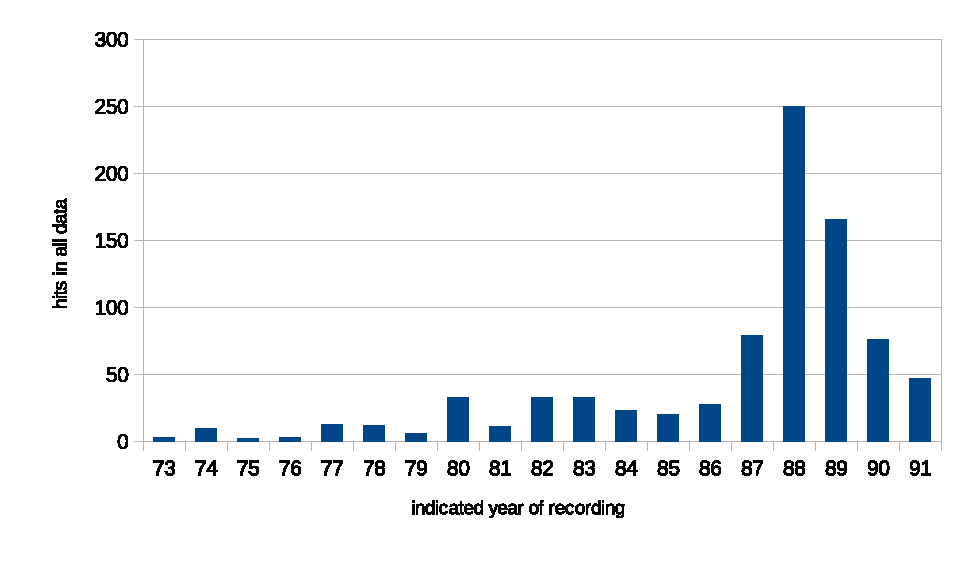
\includegraphics[scale=0.6]{rc/teresa-by-year.eps}
\caption{Number of hits for the query \texttt{terez.*} in the transcription by
alleged year of the recording}
\label{fig:teresa-year}
\end{figure}

The peak around the year 1988 supports the speculation that topics in the talks
correlate with those of books written at the same time.

\chapter{Acoustic Properties}

Automatic speech recognition is generally approached by means of machine
learning: a statistical model is inferred based on some training data. Its
application is based on the assumption that whatever was learned about the training
data will also apply to the input data. It is clear then, that if the input
data have different properties than the training data, the basic assumption is
violated and the inference performance will suffer.
Also, if the training data themselves are damaged in a way that makes the desired
information harder to extract, the learning is going to be less successful.

For speech recognition, the problem of noise, reverberation and other defects
has been a pain point and also a point of research. To mention some, Gillespie
and Atlas\cite{gillespie2002diversity} deal with reverberation for
GMM-based ASR, Yoshioka et al.\cite{reverbmagazine} summarize various
dereverberation techniques, Ko et al.\cite{reverbaugment} attempt to
simlulate reverberation in training data digitally. Seltzer, Yu and
Wang\cite{dnnnoiserobust} deal with noise in DNN-based ASR.

There are in principle two ways to deal with the negative effect of acoustic
deficiencies in speech recognition: 1) to adapt the model, which includes
training on augmented data, and 2) to adapt the input data. This chapter
presents experiments in the latter approach.

\section{ASR Performance}

We are looking into the problem of acoustic inconsistencies in terms of varying
overall quality, reverberation, noise, overdrive and other phenomena in a
dataset that is to be automatically transcribed and listened to by humans.

Te heterogenous acoustic quality of the corpus affects both the speech recognition
performance and the listening experience. Let's look at speech recognition results
of a DNN-based model trained on manually transcribed parts of the corpus, as  described in chapter~\ref{chap:svolocz}. Whereas the word error rate on the
overall test set is 19\%, it is 45\% on a sample of recordings suffering from
overdrive, and 68\% on recordings taken on a magnetophone tape with a slow
recording speed of 2 centimeters per second after some 30 years of living-room
storage.

We are conducting an experiment to make the input data similar to the training
data instead of the more usual other way around because 1) it is not easy to
make the volunteer annotators transcribe acoustically flawed data, 2) not only
speech recognition would benefit from successful denoising, the listening
experience would improve too, and 3) the model could stay leaner.

What acoustic defects are actually present? Since the corpus was digitized from
magnetophone tapes of spontaneous talks of a single speaker recorded in various
amateur conditions and with consumer devices, we can broadly distinguish these
types of quality degradation:
\begin{enumerate}
\item{additive noise -- hum or hiss,}
\item{
    stationary interference like screeching added by low-quality magnetophone
    parts or the erasing head signal,
}
\item{non-stationary interference like background speech or door slams,}
\item{
    room echo or ill-equalized microphone boosting or cutting certain
    frequencies,
}
\item{non-linear distortion of the magnetophone}
\item{speed fluctuations.}
\end{enumerate}

The individual interference types affect each other and can occur several times
in several stages. For instance, the echo is essentially convolution with a certain vector of
amplitude values, known as the impulse response. It might even not be
constant if there are moving objects in the room or if the speaker or
microphone is moving. This convolution is followed by a non-linear
distortion in the microphone and its preamplifier and convolved again with
another impulse response, this time representing a frequency and phase
response of recorder's amplifiers. Finally it is non-linearly distorted in
the process of making a magnetic recording on the tape. Another batch of
distortions comes during the playback. On top of that, in every step a certain
amount of additive noise is introduced. Clearly, modeling, let alone reverting these
interferences is a difficult task.

\section{Denoising}

We conducted a baseline experiment employing the standard denoising based on
spectral subtraction. We assumed that each recording in the
corpus suffers from a consistent kind of noise. This does not hold for all the
recordings but we dismissed this fact for the sake of simplicity. We used sox
fox the denoising routine. The process for each recording is as follows:
\begin{enumerate}
\item{Identify and isolate a sample of pure stationary noise,}
\item{extract the noise profile,}
\item{apply noise reduction based on the noise profile.}
\end{enumerate}

Items 2 and 3 are taken care of by sox. As for extracting fitting silences, we
used the following method:
\begin{enumerate}
\item{
    Identify and extract all precicted silences using an
    existing aligned automatic transcript.
}
\item{
    Select 100 silences around the 25th percentile ordered by length.
    This secures silences that are neither too short nor too long. Long silences
    tend to contain non-stationary noises, that's why we avoid using them.
}
\item{
    Create a distance matrix on the silences using
    musly\cite{schnitzer2011using}.
}
\item{
    Select 10 silences with the lowest median on the distance matrix. These
    silences are most like other silences, thus being least likely to contain
    non-speech events.
}
\item{
    Finally, catenate and output the selected silences.
}
\end{enumerate}

Subjective evaluation confirms the expectable outcome that relatively
high-quality recordings that only suffer from some additive noise get
easier to listen to. Recordings suffering from other defects and overall lower
audio quality sometimes get rather harder to understand.

We have also trained a speech recognition system on the denoised data. The
performance has sunken to word error rate of 0.94, which basically means the
transcription doesn't work at all. Probably with some parameter tweaking this
could be remedied but it doesn't seem to be a promising path. Curiously enough, the
original model trained on non-denoised data performs much better on the denoised
test data with word error rate of 0.70. Table~\ref{tab:results-denoise} sums
these up.

\begin{table}[htpb]
\caption{Word error rate for the original and denoised test data by a model trained
on the original and denoised training data.}\label{tab:results-denoise}
\centering
\begin{tabular}{|l||r|r|}
\hline
WER    & original model & denoised model \\
\hline
original testing data & 0.189 & 0.940 \\
denoised testing data & 0.698 & 0.941 \\
\hline
\end{tabular}
\end{table}

\section{Neural Domain Transfer}

The revolutionary article of Zhu et al.\cite{cyclegan} presenting
cycle-consistent generative adversarial networks gave mankind a mighty tool and
a hilarious toy that was used for de-hazing
photographs\cite{Engin_2018_CVPR_Workshops}, giving people other's facial
expressions\cite{jin2017faceoff}, in biomedicine\cite{yang2018biogan} and also
in speech processing: Kaneko and Tameoka\cite{kaneko2017parallel} present
speech domain transfer and Hosseini-Asl et al.\cite{hosseini2018malevoicegan} do
the same for the purpose of speech recognition.


Most closely related to the work presented in this article is probably
SEGAN\cite{pascual2017segan}: CycleGAN employed to enhance speech.

CycleGAN assumes two datasets in consistent domains: day and night photos,
schematic and photographic maps, male and female speech etc. In this case,
we have a clear consistent domain of clean, high-quality recordings and the
rest, which suffers from any combination of a number of defects. The damaged
recordings are very unlike each other, they don't form a consistent domain.

There are two ways of dealing with this situation: 1) adapt CycleGAN so that it
can deal with a ``compact'' and a ``scattered'' domain or 2) cluster the
data and apply CycleGAN on the individual clusters. While adapting CycleGAN may be a
point of future work, we have explored the simpler way of clustering the data.

\section{Clustering}

In order to perform clustering on any dataset, a metric on the data is needed.
We have used that proposed by Mandel \& Ellis\cite{mandel2005song}, which
is based on mel-frequency cepstra. A distance matrix has been created using
musly and the clusters on top of that using
hierarchical clustering\cite{johnson1967hierarchical}.

A manual... or rather aureal check on the clusters confirms that files falling
into a cluster are indeed acoustically similar. So we arrived at a cluster of
overdriven recordings, a cluster of heavily hummed ones etc.

For curiosity, we looked at the distances of the files among each other and
compared it to that between other familiar sounds. For instance, two adjacent
segments of the same speaker from a meeting of the Czech parliament has a
distance of 1.4. Different speakers have a distance of 6.5. One of these
segments compared to a black metal song chorus has the distance of 519. On the
other hand, the median distance among the Spoken corpus of Karel Makoň, where
there is a single speaker, amounts to 55.9.

The experiment presented below is conducted on three clusters:
\begin{enumerate}
\item{A cluster of the cleanest recordings, used as the destination domain,}
\item{a cluster of overdriven recordings and}
\item{a cluster of recordings taken with low tape speed.}
\end{enumerate}
Recordings in cluster 3 are the hardest to understand even for humans. All these
clusters have a maximum internal distance of 25.

\section{Results}

We have used the voice transfer method as proposed by Kaneko \&
Kameoka\cite{kaneko2017parallel} and implemented by
Mao\footnote{github.com/leimao/Voice\_Converter\_CycleGAN}. We have trained
transfer 1) between the clean and the overdriven cluster and 2) between the
clean and the low-speed cluster.

After 200 epochs, we have performed speech recognition on the transferred data.
The result is summed up in Table~\ref{tab:results}.

\begin{table}[htpb]
\caption{Word error rate for the two damaged clusters before and after CycleGAN
transfer.}\label{tab:results}
\centering
\begin{tabular}{|l||r|r|}
\hline
           & original & transferred \\
\hline
overdriven & 0.450 & 0.441 \\
low-speed  & 0.685 & 0.939 \\
\hline
\end{tabular}
\end{table}

The word error rate decrease in the overdriven cluster is unfortunately statistically
insignificant with standard deviations 0.054 and 0.079 of the transferred and
original versions respectively. An important benefit is
that the transferred overdriven (or should we say de-overdriven) sound files are
much easier on the ear and it can be a help for human listeners.

The wrecking word error rate increase from 69\% to 94\% in case of the
recordings taken at low tape speed requires further investigation.
Figure~\ref{fig:plzen} shows the waveform and spectrum of a sample from the low-speed
cluster before and after the transfer. For comparison,
Figure~\ref{fig:overdrive} shows the same for the overdriven cluster.
Notice how parts of the signal are completely missing in the converted low-speed
sample. It seems that when the signal is too hard to separate from the noise,
the convertor prefers to generate silence.

\begin{figure*}[tpb]
\centering
\includegraphics[width=0.9\hsize]{rc/plzen.eps}
\caption{Wave form (above) and spectrogram (below) of a recording taken in low
tape speed before the CycleGAN transfer (left) and afterwards (right).}
\label{fig:plzen}
\end{figure*}

\begin{figure*}[tpb]
\centering
\includegraphics[width=0.9\hsize]{rc/overdrive.eps}
\caption{Wave form (above) and spectrogram (below) of an overdriven recording
before the CycleGAN transfer (left) and afterwards (right).}
\label{fig:overdrive}
\end{figure*}

\chapter{Speech Recognition on Makoň's Corpus}
\label{chap:svolocz}

Acquiring a complete transcript of the given speech recordings is a central task
of this thesis. Furthermore, the method proposed assumes an initial transcript
to be present from the beginning. Therefore, developing a speech recognition
system for the data at hand was an ubiquitous task for me.

I have built the first system using HTK and have later switched over to
DeepSpeech, a system based on deep neural networks inspired by the 2014 Baidu
article\cite{hannun2014deep}.


Training data for speech recognition is always a demanded commodity, especially
if it is free. There are for sure already some free Czech corpora fit for speech
recognition training:
\begin{itemize}
\item{
    Vystadial\cite{vystadialarticle} with its 77 hours of VoIP
    calls\cite{vystadialdata}, 
}
\item{
    The Prague Database of Spoken Czech\cite{pdtscarticle} with its 122 hours
    of richly annotated spontaneous dialogues\cite{pdtscdata},
}
\item{
    The Czech Senior COMPANION Expressive Speech Corpus with its 5 hours
    of professionally spoken utterances by a single speaker\cite{companiondata},
}
\item{
    Otázky Václava Moravce: 35 hours of transcribed recordings of the
    Czech TV talk show\cite{ovmdata},
}
\item{
    STAZKA, a set of speech recording from vehicles with its 35 hours of
    background noise and utterances\cite{stazkadata},
}
\item{
    Spoken Corpus of Karel Makoň\cite{kruuza2012making} with its 100 hours of
    manually transcribed spontaneous speech by a single speaker\cite{makondata},
}
\item{and possibly others that I am not aware of.}
\end{itemize}

The Czech parliament meeting recordings represent a publicly available dataset
of high-quality audio recordings of contemporary Czech in consistent low-noise
audio quality worth almost 4000 hours of downloadable material, about 2800 hours
after subtraction of the overlaps. Extracting
training data for speech recognition systems would provide a corpus at least
one order greater in length than those so far publicly available.

Verily, I am not the first person to attempt using these recordings for speech
recognition. The Department of Cybernetics of University of West Bohemia
developed an automatic online subtitling system for the meetings in
2006\cite{pspsubs} and as a result, an 88-hour subset annotated by high-quality
automatic transcript has been released for speech recognition training
purposes\cite{pspdata}.

I attempt to use the official stenographic transcripts available for all the
talks so that it can be a new entry in the above list, on par in quality and
excelling in size.

\section{Data Preparation}

Since the source data is publicly available and in the public domain, I merely
provide the scripts for downloading and building the corpus. The algorithms and
parameters used are described in this section.

\subsection{Scraping}

Regrettably, the data are to my best knowledge only available in human-readable
form. The transcript is not clearly distinguished in the markup and is
interlaced with metainformation. My method of isolating the transcript is quite
crude but it covers the vast majority of cases. The criterion is to extract the
subtree of all nodes with HTML attribute \texttt{[align=justify]}, except HTML
elements \texttt{<b>}, which contain speaker identification.

The known shortcomings of this method are that 1) it discards the speaker
annotations, although it is valuable metainformation and 2) it skips some short
passages, e.g. references to other meetings, as can be seen in the meeting
from Feb. 12th 2020 10:10 -
10:20\footnote{https://www.psp.cz/eknih/2017ps/stenprot/040schuz/s040372.htm}.
Both can be corrected by devising a smarter scraper and neither has any
significance for speech recognition: speaker annotation fundamentally and
neglecting the links for their infrequency.

\subsection{Alignment}

One of the obstacles in using the stenographic transcripts for training an ASR
system is the very loose alignment available. The recordings are all 14 minutes
long and have a 4-minute overlap. The corresponding transcript is thus aligned
in 10-minute blocks with a roughly 2-minute padding on each side of the audio.
Figure~\ref{fig:overlap} schematically shows the alignment of the stenographic
transcript to the audio and the overlap of the recordings.

\begin{figure*}[tpb]
\centering
\includegraphics[width=0.9\hsize]{rc/overlap.eps}
\caption{Alignment and overlap of audio files and transcript. The examples are
from Feb. 12th 2020 around 10 o'clock. The transcript corresponding to the
recording in the upper left covers audio positions 01:34 - 11:24. The one in the
lower right from 01:24 to 12:00.}
\label{fig:overlap}
\end{figure*}


Systems for aligning long audio segments to their transcripts already exist,
like that of Moreno et al.\cite{moreno1998recursive} or
Hazen\cite{hazen2006automatic}. They are both based on an already existing
automatically acquired transcript. I use this technique as well, though 
simplified and adapted to the task.

I have used the dataset mentioned above\cite{pspdata} to train a GMM-based ASR
system, using the stenographs as training data for a language model. Using these
models, a word-level-aligned transcript of the whole set of recordings has been
acquired.

The predicted transcript and the stenographic one have then been compared for
Levenshtein distance, determining the edit operations needed to transform one
into the other. For each predicted word, a reliability score is then
computed as 1 - unreliability where unreliability is the number of edit
operations taken on it divided by its length.
Figure~\ref{fig:align} shows how the stenographic transcript is aligned with the
audio on word level.

\begin{figure*}[htpb]
\includegraphics[width=0.9\hsize]{rc/align.eps}
\caption{Schema of aligning the audio to the stenographic transcript on word
level.}
\label{fig:align}
\end{figure*}

Nota bene, a GMM-based system was chosen for the initial transcript instead of
a DNN-based for three reasons: 1) Foremost, it is straightforward to obtain
precise alignment from a GMM-based system. 2) The training doesn't require so
much computational resources and data. 3) It isn't crucial to have maximum possible
accuracy in this stage.

\subsection{Audio Segmentation}

To create a usable dataset for training a speech-to-text system, it is not
necessary to perfectly align the whole transcript. On the contrary, it is
desirable to align what is reliably precise and discard the rest.

The criteria for good training samples are:
\begin{enumerate}
\item{100\% precise transcript,}
\item{roughly sentence-level length,}
\item{consistent length.}
\end{enumerate}

To ensure precise transcript, it is good to have the samples padded by some
silence, since the alignment obtained from the initial ASR may be a bit
imprecise. We thus want to split at pauses, the longer the better, up to a
certain limit (about 1 second). The need to split at longer
pauses goes against the need to split at consistent, none-too-great lengths.

So the problem is to select an optimal set of silences so that the longest ones
are used and so that they split the recording into chunks of length in a given
range. This looks like a problem for dynamic programming but a simpler approach
is also possible: Start with a set of all silences predicted by the forced
alignment.  Iterate over the silences shortest-first and remove each if it
doesn't break the constraints.

I have experimentally set the length boundaries to 12 - 30 seconds. The maximum
length could be decreased at the cost of available pauses to choose from, which
would lead to more frequent splits in the middle of a word.

\subsection{Training Samples Selection}

With the audio segmented and corresponding manual transcripts extracted, the
last step remaining is selecting which segments to include in the traning data.
Indeed, since the recordings have a 2-minute padding on each side for 10 middle
minutes, we must discard at the very least 40\% of the segments. I use the
following criteria for including a segment in the data:

\begin{enumerate}
\item{The first and last token have reliability at least 70\%,}
\item{The mean reliability of all tokens is at least 70\%,}
\item{The number of words is no less than five.}
\end{enumerate}

Minimum reliability of border tokens is considered to minimize the danger of
shifted alignment boundaries. Mean reliability is considered because it is OK
for some words to have very low reliability: there are enough errors in the
prediction, that's why we use the manual transcript after all. But if too many
tokens have too low reliability, then it is a sign of a suspicious segment. The
number of words has a minimum because with only a few words, the probability of
misalignment with good score is much greater than when there are enough words.

Why use mean reliability and not median? The way the reliability is computed
considers the number of edit operations on one line in the automatic transcript.
In the case where there are many insertions, the reliability of one line can go
arbitrarily deep sub zero. So it can happen that there are several inserted
words in a (mis)aligned chunk that only affect the reliability score of a single
word. The mean taps these while the median doesn't.

\subsection{Data Extraction Summary}

All the constants and criteria are to be considered a baseline solution. They
all could be tweaked much more rigorously and solved much more soundly. However,
this simple solution readily yields a high-quality training dataset of 1058
hours. Of the total 539,057 segments, 142,530 (26\%) have been accepted to the
training dataset. Of the total 396,527 discarded segments, 350,258 (88\%) were
discarded because of the criterion of unreliable start or end. It should be
noted however, that the start / end reliability criterion is applied first, so
it catches segments that would be discarded for other reasons also.

Reducing the minimum reliability of the boundary words from 70\% to 50\% increases
the number of accepted chunks by 17\%. It adds 5\% segments
of the total number to the dataset. But if we consider that 40\% of the total
number of segments must be discarded because of audio padding, the gain is
acually 9\%. It is an option to increase the training data volume at the cost
of matching precision.

\section{Numerals and Abbreviations}

There are many numeral expressions in the transcripts. They amount to 489,880
out of 25,010,269 tokens in the complete stenographic transcript, which is
almost two percent. In the training dataset, 24\% of the samples contain one or
more numerals.

Originally, I have included the digits into the alphabet for speech recognition,
thus attempting to train the system to transcribe numeral expressions directly
into digits. The speech recognition system described in the following section
would however transcribe numeral expressions as empty strings.

There are four ways to deal with the problem:
\begin{enumerate}
\item{ignore it,}
\item{remove digits from the training data,}
\item{manually expand digits to words,}
\item{automatically expand digits to words.}
\end{enumerate}

The first option needs no elaboration. The second one, removing samples with
digits, is an easy and viable option but it is a waste of a quarter of the
dataset and of the vast majority of samples with numerals in them. Manual
expansion would surely be ideal but very costly. It remains to attempt the
fourth variant of automated expansion.

For automated expansion of digits into words, we can use the available initial
transcript and the algorithm for alignment with the stenographic transcript.

The expansion is done in two steps:
\begin{enumerate}
\item{generation of verbal variants,}
\item{selection of the most likely variant.}
\end{enumerate}

I have used the Perl module \texttt{Lingua::CS::Num2Word} as a base for the
expansion. I modified the module in the following way: 1) I added support for
the order of billions, which is very common in the corpus. 2) A number is no
longer expanded into a single phrase but instead into all possible phrases
expressing the given number. 3) I added support for genitive and accusative
cases, decimal numerals, ordinals, dates and times.

All tokens in the stenographs that include digits are expanded into their
verbalization variants before further processing. Upon alignment, the variant
with least edit distance from the initial transcript is selected.

Common abbreviations and symbols are expanded together with the digits. For
example, the very common character \textit{``§'' (paragraph)} is expanded into
the forms \textit{paragraf, paragrafu, paragrafů, paragrafem,
paragrafech} that represent common inflections of the word. Some common
abbreviations that undergo inflection include \textit{``čl.'' (article)},
\textit{``odst.'' (also paragraph)} and \textit{``tzv.'' (co-called)}.

After incorporating the expansion into the pipeline, the similarity of the
stenographic transcript and the initial one raised, which also raised the number
of accepted segments from 26\% to 35\%. The amount of training data grew by 86
hours to 1144.

\section{ASR Based on the Dataset}

I have trained a standard DeepSpeech\cite{hannun2014deep} model on the 1058
hours with training :
development : test ratio of 18 : 1 : 1; batch size 50; learning rate 0.0001; dropout
rate 0.2. The training took 12 epochs to reach optimal dev fit and the final
word error rate on testing data from the corpus itself is 8.40\% before digit
expansion and 7.89\% afterwards.

The language model used was a pentagram model with pruned singleton trigrams,
tetragrams and pentagrams. The bulk of scraped transcriptions, including those
with no downloadable corresponding audio, was used as training data for the
language model.

I have also tried training a speech recognition system with other datasets and
the combination of them all. Of the datasets listed in
section~\ref{sec:intro}, only Vystadial, Otázky Václava Moravce (ovm) and the
corpus of Karel Makoň (makon) proved useful without much effort.

Apart from them, I used the publicly not available corpora of Charles University
Corpus of Financial News (CUCFN, 65 hours)\cite{byrne1999large}, the Balanced
corpus of informal spoken Czech (Oral2013, 293 hours)\cite{oral2013} and the
spoken Bible (100 hours) available with no license terms from
\url{poslouchamebibli.cz}. Table~\ref{tab:csasr:results} shows the speech recognition
results for each corpus on test data from itself and on a common test set from
all the corpora.

\begin{table}[htpb]
\caption{Word error rate of speech recognition on the individual corpora and on
their concatenation.}
\centering
\begin{tabular}{|l||r|r|}
\hline
source    & WER on self & WER on all \\
\hline
bible     & 9.20\%  & 94.7\% \\
cucfn     & 31.6\%  & 72.8\% \\
makon     & 30.4\%  & 77.3\% \\
oral2013  & 78.4\%  & 60.7\% \\
ovm       & 21.6\%  & 72.9\% \\
parliament w/digits
          & 8.74\%  & 39.7\% \\
\textbf{parliament expanded}
          & 7.89\%  & \textbf{36.0\%} \\
vystadial & 51.0\%  & 74.0\% \\
\hline
all w/digits & 28.4\% & 28.4\% \\
all expanded & 26.0\% & 26.0\% \\
\hline
\end{tabular}
\label{tab:csasr:results}
\end{table}

All speech recognition systems were trained with the same hyperparameters as
described above.

\chapter{Web Interface}

The spoken corpus is about 1000 hours of a single
speaker. Our aim is to have a transcription as good as possible for the purpose
of searching and further, higher-level processing of the data. There is a pool
of people interested in the talks, who on one hand are the force we can try to
employ and on the other hand are the consumers of our effort, our target group
so to speak.

The web application should therefore combine the two purposes: 1. serve its user
with making the content available in a manner as good as possible and 2. animate
the user to give as much and as high-quality contribution as possible.

To our best knowledge, there is no other project with a comparable setting.
However, we can compare single aspects found in other applications.

\subsection{Transcription Apps}
\label{ssec:diff:trans}

The best widespread match to our task is that of creating an application for
transcribing speech recordings. Let us compare the two tasks, pointing out the
main points of difference. For reference, we take (1)
Transcriber\footnote{trans.sourceforge.net}, a classical open-source program
written in TCL, (2) oTranscribe\footnote{otranscribe.com}, a free modern
web-based transcription tool and (3) Transcribe\footnote{transcribe.wreally.com}
a commercial web-based transcription tool.

The numbers in the bullet list below denote the programs our statement applies
to. For example, of the three only Transcriber allows speaker annotation, hence
there is only the number (1) standing at the second list item.

\noindent
\begin{tabularx}{\textwidth}{
    @{\hspace{1.5em}}% Space for left bullet
    >{{\hsize=0.9\hsize}\leavevmode\llap{\textbullet~}\raggedright}% Left bullet + formatting of column
    X% Left column specification
    @{\hspace{0.2em}}
    >{\hsize=0.2\hsize}
    X
    @{\quad\hspace{1.5em}}% Space between columns + right bullet space
    >{\leavevmode\llap{\textbullet~}\raggedright\arraybackslash}% Right bullet + formatting of column
    X% Right column specification
    @{}% No column space on right
  }
  \em{transcription applications}: & & \em{our application}: \\
  are optimized for the case where there is no transcription available and it
  must be acquired from scratch; &
    (1,2,3) &
      always assumes a prior transcription is available; \\

  allow annotation of speakers; &
    (1) &
      assumes all utterances come from the same speaker; \\

  need no quality control: the user is free to enter whatever transcription she
  pleases and the ultimate measure is her satisfaction; &
    (1,2,3) &
      needs the transcription to be accurate because it is used as training data
      for the acoustic model; \\

  use alignment on the level of phrases, if any; &
    (1)\footnote{
        Transcriber explicitly aligns the text with speech, while the
        other two merely support addition of timestamps into the transcription.
    } &
      uses alignment on the level of words; \\

  are user-centric: the user transcribes whatever acoustic data they choose; &
    (1,2,3) &
      is data-centric: the whole application with all its tools and persons
      revolves around the data set; \\

  assumes the user wants to transcribe; &
    (1,2,3) &
      assume the user wants to listen and possibly read along and we want to
      animate her to submit transcriptions; \\

  has no shared data between users; &
    (1,2)\footnote{Transcribe supports team co-operation.} &
      must count with collisions. \\
\end{tabularx}

\vspace{5mm}

Despite of these differences, we can still learn a lot from transcription
software. The ease of performing common tasks, like pausing, resuming and
rewinding is crucial for the user experience and in effect for the amount of
submissions that we receive. Also, the way the text is displayed synchronously
to the audio played has a big impact and the approaches have a lot of space for
variation.

\subsection{Wiki}

Where our application diverts from transcription software, it mostly resembles a
wiki: a community platform that serves its users including the contributors but
where the quality of the contributions is essential, while the contributor's
satisfaction alone is of less importance.

One major point of difference to a wiki is that wiki is creative, whereas our
task is mechanical. The user has basically no room for their own invention:
providing a different than correct transcription is seen as an error.

Popular wikis have good measures for edit conflicts, which is where we could
learn some lessons. However, so far there was no need to do that because
\begin{enumerate}
\item{if we always simply take the most recent version
of a segment, the result stays consistent even if a piece from user A comes into
a larger transcription of user B;}
\item{our user base is so far limited to a small community who have no problem
coordinating with each other. We plan to expand to broader public soon though.}
\end{enumerate}

With regard to the transription as presented to the user, a submitted segment of
transcription always overwrites the present version but we keep all the
submissions in a database, so undo operations, clustering submissions by their
author etc. are possible but we had little need for this so far.

\subsection{Corpora}

Our project is not the first involving community-driven care of a corpus. We
can mention the Manually annotated sub-corpus\cite{ide2010manually}, where
annotations of various kinds are gathered from volunteers, or the
Wikicorpus\cite{reese2010wikicorpus}, a corpus of Wikipedia articles with some
linguistic annotation. Our project may reach profound similarities with these in
the future, when we no longer focus on the transcription itself but rather on
annotation.

There is also CzEng\cite{bojar2008czeng}, the Czech-English Parallel
Corpus, where a large part of the translation is provided by volunteers. The
similarity in setting is considerable as both projects involve a
machine-produced erroneous derivative of the original material (in our case
audio transcriptions, in the case of CzEng Czech translations of English texts),
and a community of volunteers correct these. But the specifics of the projects
bring different challenges and dictate different approaches.

Marge (2009)\cite{5494979} investigates using The Mechanical Turk to obtain
audio transcriptions. Mihalcea (2004)\cite{mihalcea2004building} offers a web
interface for word-sense disambiguation and focuses mostly on annotator conflict
resolution.

\section{Description of the Web Application}

\subsection{Usage}

We have no special assumption of the user beyond basic computer usage skills and
understanding the audio. We assume no prior training. There is a manual for
clearing common points of confusion. The main message in it is that anything
that is to be transcribed, should be transcribed with respect to
phonetic precision, even if it results in nonsensical character strings.

Anything except words spoken by the one speaker of interest is to be left
untranscribed, including noise or speech by other persons\footnote{In our data,
other speakers represent a negligible fraction but we may later add support for
speaker annotation.}. Incomprehensible words are to be left uncorrected
(the ASR output kept) if the phones are unclear. If the phones uttered are clear
but it is not clear what word was meant, the word may be transcribed
phonetically.

\subsection{Implementation}

The application consists of several views:
\begin{enumerate}
\item{the start page where all recordings are listed and each points to a detail
view,}
\item{the detail view, where a recording can be played back, its transcription
is displayed and can be corrected by the user,}
\item{the search page, where hits to a search query are listed and point to
corresponding positions in the recordings,}
\item{static pages with general information, contact etc.}
\end{enumerate}

We shall only discuss the detail view as the others are not relevant to this
paper. Figure~\ref{fig:scn1lab} shows the interface during playback.
Figure~\ref{fig:scn2lab} shows the interface while a segment is being edited.
The interface in the figures is conveniently shown in English, although in
reality it is in Czech.

\begin{figure}[htpb]
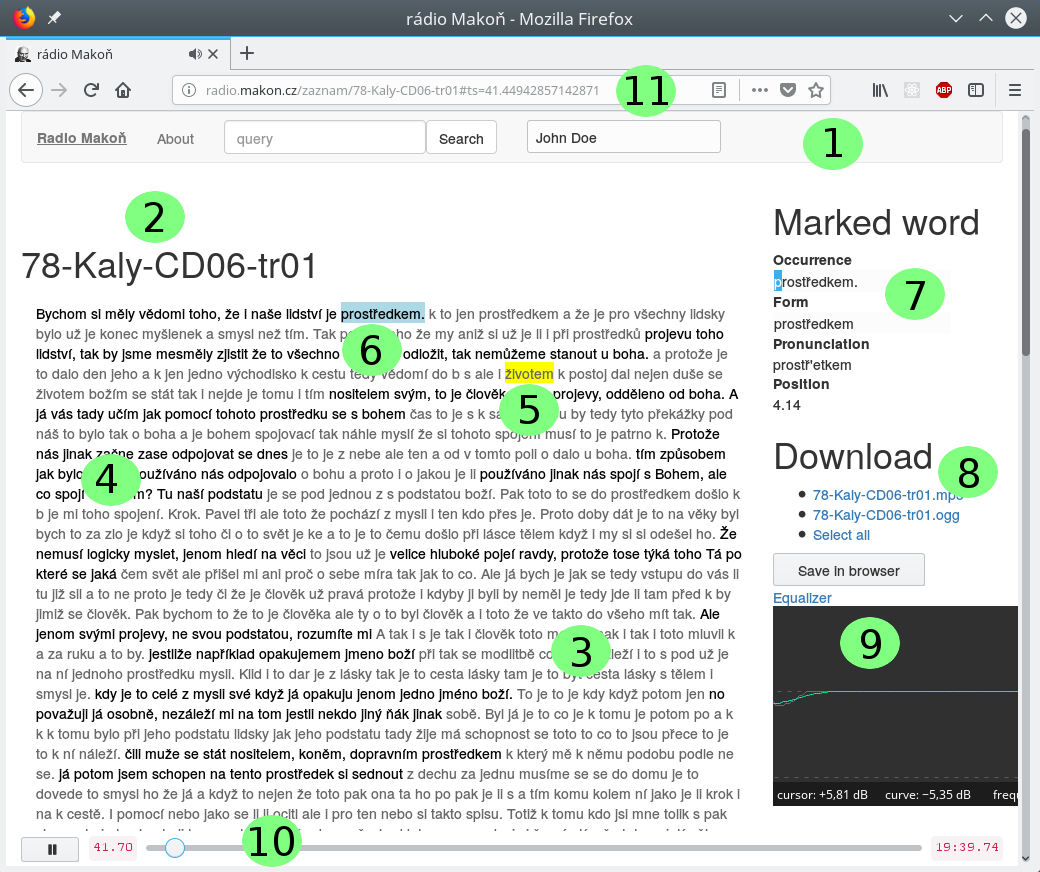
\includegraphics[scale=0.6]{rc/radio-makon-en-1-lab.png}
\caption{Web interface during playback}
\label{fig:scn1lab}
\end{figure}

Legend to Figure~\ref{fig:scn1lab}:
\begin{enumerate}
\item{
    Header with
    \begin{itemize}
    \item{app name linking to start page,}
    \item{about link,}
    \item{search field and}
    \item{username input field;}
    \end{itemize}
}
\item{Identifier of the recording;}
\item{Automatically transcribed segments in grey;}
\item{Manually transcribed segments in black;}
\item{Currently played-back word highlighted by yellow background;}
\item{Marked word highlighted in regent st. blue;}
\item{
    Marked word info:
    \begin{itemize}
    \item{
        occurrence: the word with contextual capitalization and
        punctuation as it appeared in the text (currently being edited as the
        selected initial letter reveals),
    }
    \item{form: normalized word form as it appears in the word list,}
    \item{pronunciation: Czech phonetic transcription of the word,}
    \item{
        position: time of the beginning of the word in seconds from the
        start of the recording;
    }
    \end{itemize}
}
\item{
    Tools for storing:
    \begin{itemize}
    \item{direct links to the audio files,}
    \item{selecting the whole transcription for easy pasting,}
    \item{storing the decoded recording in the browser's IndexedDB;}
    \end{itemize}
}
\item{Graphical equalizer for compensating narrow-band noise;}
\item{
    Audio playback controls:
    \begin{itemize}
    \item{play/pause button,}
    \item{current playback position,}
    \item{playback scrollbar,}
    \item{total recording length;}
    \end{itemize}
}
\item{Current position reflected in URL fragment.}
\end{enumerate}

\begin{figure}[htpb]
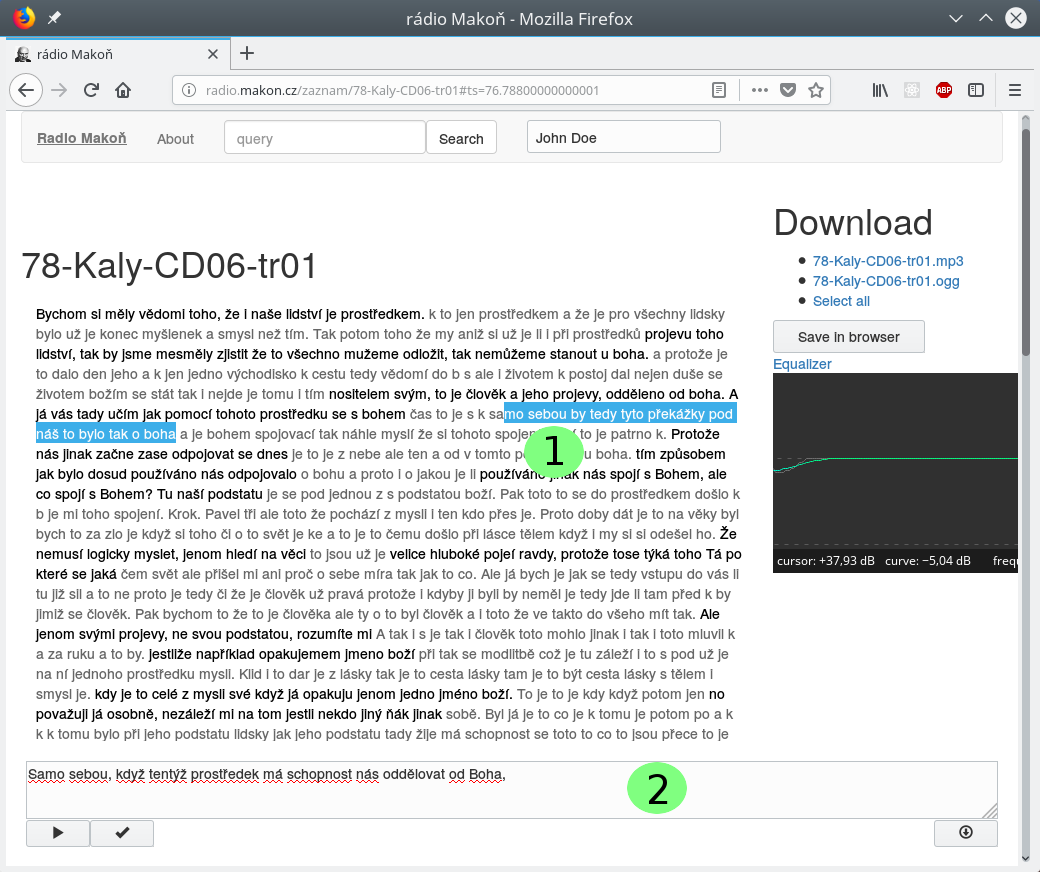
\includegraphics[scale=0.6]{rc/radio-makon-en-2-lab.png}
\caption{Interface in the state of editing a segment}
\label{fig:scn2lab}
\end{figure}

Legend to Figure~\ref{fig:scn2lab}:
\begin{enumerate}
\item{
    Selecting a text range with the mouse defines the segment the user is about
    to transcribe;
}
\item{
    The edit tool with
    \begin{itemize}
    \item{text area prefilled with the current transcription,}
    \item{playback button that plays the corresponding segment,}
    \item{save button and}
    \item{download-segment button, which initiates a file-save action for the
    audio segment corresponding the the selected text. The synthesis of the
    downloaded file takes place in the browser.}
    \end{itemize}
}
\end{enumerate}

The commonest tasks have keyboard shortcuts: \texttt{ctrl+space} for
play/pause and \texttt{ctrl+enter} for submitting a correction.

\subsection{Displaying the Transcription}

Many transcription programs show the transcription as a vertical list of
utterances, see Figure~\ref{fig:transcriber1} for an example of
Transcriber. We attribute this to the fact that the atomic elements of
the transcription are the user-entered utterances and their boundaries are
reliable. In our case, the atomic elements are words. There are sentences, sure,
but the segmentation to sentences by the ASR is very unreliable, so we want it
to be natural to transcribe a segment overlapping sentence boundaries.

\begin{figure}[htpb]
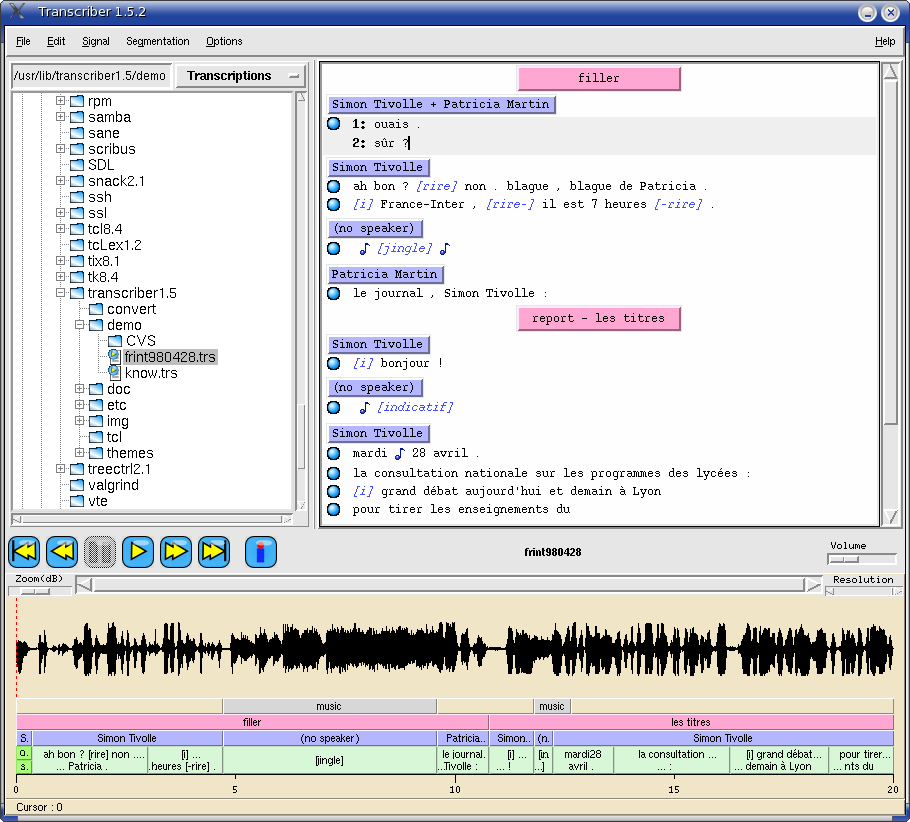
\includegraphics[scale=0.4]{rc/transcriber1.png}
\caption{A screenshot of Transcriber}
\label{fig:transcriber1}
\end{figure}

This is one of the reasons why we display the transcription basically as a
single wrapped line.

\subsubsection{Performance Challenge}

The transcription display was designed to have these features:
\begin{enumerate}
\item{
    Currently played-back word should be highlighted;
    \label{feats:item:curword}
}
\item{
    Manually transcribed segments should be clearly distinct from automatically
    transcribed ones;
    \label{feats:item:manualdistinct}
}
\item{
    Selecting one or more words with the mouse should trigger transcription mode
    for the selected text;
    upon a successful save, this should be merged into the display;
    \label{feats:item:selectable}
}
\item{
    Clicking a word should bring up its context info (we call this the
    {\em marked word} as the term {\em selected word} is already taken);
    \label{feats:item:clickable}
}
\item{
    The whole transcription should be shown at once for easy searching;
    \label{feats:item:showall}
}
\item{
    The page should be responsive.\label{feats:item:speed}
}
\end{enumerate}

These requirements are harder to combine than it may seem. Notably
responsiveness is hard to combine with all of the other ones. Why is that so?

Points~\ref{feats:item:curword} through \ref{feats:item:clickable}
call for every word to be wrapped in its own element.
Point~\ref{feats:item:showall} and the median count of words in a transcript of
about 6000 yield 6000 \texttt{<span>} elements just to show the text. 

Although this may not seem like a big deal, it does affect the responsiveness
and memory footprint of the page.

In the original version, we solved this by sacrificing point~5:
only 3 lines of text are shown with the current word kept on the middle line as
shown on Figure~\ref{fig:makonfm}.\footnote{The current word is on the top line
on the screenshot because it is at the beginning of the recording.} Thanks to
the development in the web standards and their support from popular browsers, a
solution is possible.

\begin{figure}[htpb]
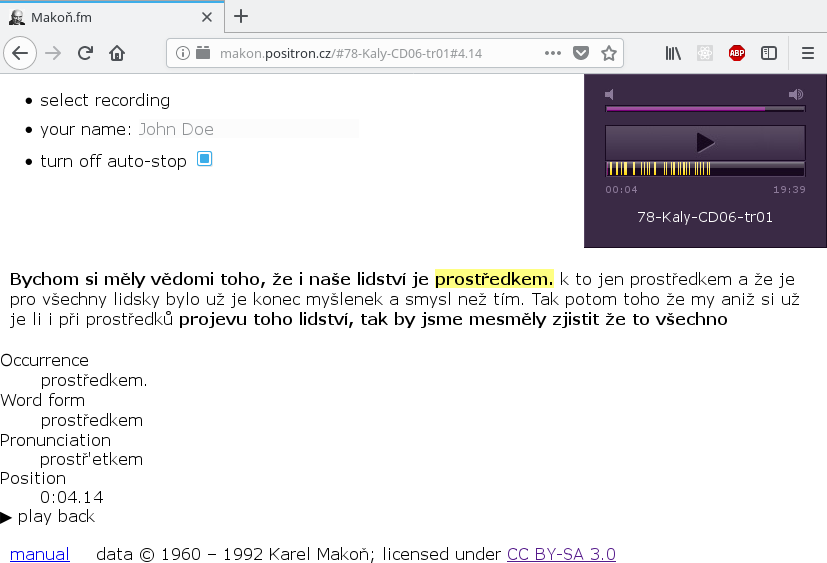
\includegraphics[scale=0.7]{rc/makonfm-en-1.png}
\caption{Original web interface from 2012}
\label{fig:makonfm}
\end{figure}

\subsubsection{Solution}

We can use the fortunate fact that manually transcribed words and automatically
transcribed ones tend to form larger chunks. The average number of words per
submitted segment is 7.9. Furthermore, the absolute majority of such segments
are adjacent to other manually transcribed chunks.\footnote{
The median number of chunks is 1 (most recordings have no manually corrected
segments), maximum is 1109. Median only counting touched recordings is 8.}
Hence, wrapping each chunk of consecutive manually or automatically transcribed
words in an HTML element is no problem, which solves
point~2.

Point~\ref{feats:item:selectable} can be implemented using
\texttt{document.selection} and the \texttt{Range} objects, which let us find
out the innermost HTML element and text offset of the start and end of the
textual selection. Since we know the length of each word, this allows us to map
the selection to the corresponding words in the transcription.

Points~\ref{feats:item:curword} and~\ref{feats:item:clickable} can be
implemented in two ways: We could either wrap the current and marked word in a
dedicated element or we could draw a highlighting rectangle beneath the word.

Wrapping the word would definetely be more robust and less error-prone but the
constant changes in the DOM during playback with possible frequent reflows speak
against it. Finding the exact position of each word and drawing a rectangle
precisely beneath it (beneath on the z-axis; over it in the x-y sense), avoiding
positioning issues and keeping the rectangle position synced even after scrolling
/ window resizing is definitely a challenge but we chose this way nonetheless.
The performance gain for the majority of the usage time outweighs the possible
errors in the corner cases, more so since the eventual errors are not critical
and mostly remedied by further playback.

The efficiency of repositioning a rectangle is supported by the fact that we can
calculate the coordinates of all rendered words once and only recalculate them
in two cases: 1) In the rare event of screen resize and 2) when a corrected
segment is merged into the transcription, in which case we only need to
recalculate for the words further in the document.\footnote{We could even stop
the recalculation as soon as we find that the new horizontal coordinate of a
word is left untouched, and add the difference in the vertical coordinate to all
subsequent words, i.e. when a line stays the same, so do all below it.}

\subsubsection{Manual / Automatic Distinction}

As shown on Figure~\ref{fig:scn1lab}, we draw automatic transcription in grey
and manual one in black. Why did we choose this instead of normal / boldface?
Firstly, the normal font is optimal for reading. Boldface is meant to highlight
spots in text. It becomes bulky when applied on long continuous passages. The
automatic transcription contains many errors, so there is no sense in optimizing
it for best reading experience.

There is also another practical reason. When the two font variants only differ
in color, and a segment of automatic transcription is left intact and submitted
as correct transcription, its merge-down into the displayed text causes no
reflow, which saves us computations and raises responsiveness. It may seem like
a rare use case but we believe that identifying correctly recognized words is a
legitimate way of contribution, so why not optimize for it?

Still, the underlying HTML tags are \texttt{<span>} and \texttt{<b>} because
that way the distinction persists when copy-pasting the text from the web page
to a rich text editor.

\subsection{Ergonomy}

It is clear that the ease of use is crucial in our case where the user is
supposed to perform a requiring, tedious task with repeated steps, especially
since it is our interest more than hers that she performs them. We compared our
setting with that of transcription apps in section~\ref{ssec:diff:trans},
pointing out lessons to learn. Let us now look at some specific points and their
actual (lack of) implementation.

\subsubsection{Keyboard Shortcuts}

One of the most profound measures in ergonomy are keyboard shortcuts. The most
common task is pausing and resuming playback. Both oTranscribe and Transcribe
use the \texttt{esc} key for that, and Transcriber uses the \texttt{tab} key.
We chose \texttt{ctrl+space} combination. We argue that \texttt{esc} is not the
best of options for desktops because the distance the fingers have to travel
from the alphanumeric keys causes a noticeable delay. This can lead to missing a
pause between words. The \texttt{tab} key as chosen by Transcriber is a splendid
choice from the ergonomy point of view and there is no reason not to use it in a
dedicated user interface. However, in the browser, where the \texttt{tab} key
has as native use, re-binding it could lead to confusion and irritation. The
space bar is probably the easiest-to-find key in all situations and dedicating
\texttt{ctrl} to all application-specific commands as opposed to single keys
lends a sense of consistency, we believe.

This is mere personal experience though, as we had no resources so far to
perform serious research to support these statements.

The only other keyboard shortcut we support is \texttt{ctrl+enter} for
submitting the correction. We chose this to stay consistent using the
\texttt{ctrl} key and because this shortcut is familiar to users of many instant
messengers, like the Facebook chat or the once popular official ICQ client.
Also, requiring a key combination prevents accidental submission, which is
desirable as we only want double-checked, guaranteed-precise ones. In
comparison, Transcriber uses the bare \texttt{enter} key to separate utterances.
oTranscribe and Transcribe allow free formatting with no explicit alignment, so
using the enter key to split utterances by lines is the user's choice.

\subsubsection{Missing Features}

One of the features that Transcribe, the only commercial tool in our reference
list, offers is setting up keyboard shortcuts for common words. We have not
implemented this because ideally, common words should be covered by speech
recognition. However, it could be sensible to implement it anyway. The reason is
that a word can be very rare globally and thus poorly recognized by ASR but very
common in a specific passage. This particularly regards named entities.

Another point in our ergonomy to-do list is lifting the need to select a segment
prior to correcting it. If the transcription was simply editable, it could
increase the ease of use rapidly. We would have to automate the selection of
segment to send for forced alignment but we could probably do a better job than
the user in the end.

\subsection{Mechanics of Submitting a Corrected Segment}

As stated above, when the user selects at least one character with the mouse,
the application enters the state of correcting the selected transcription padded
to whole words. In this mode, the transcription to correct is shown in a
text area and the global playback controls are replaced by those that only allow
playback of audio corresponding to the selected transcription.

Once the user believes that the content of the text area corresponds precisely
to the words uttered, she hits the {\em save} button or the \texttt{ctrl+enter}
keyboard shortcut. This starts an asynchronous HTTP request to the back-end,
where parametrized (MFCC) versions of the recordings are stored, along with the
new transcription and the time positions of the beginning and end of the
segment.

The server then cuts off the corresponding segment from the parametrized
recording, runs forced alignment on it with the provided transcription with a
threshold to reject bad matches. If the forced alignment fails, an error
response is sent back and the transcription is not merged into the original. In
the case of a success, the correction is merged on one hand on the server side
and pushed to a CDN, on the other hand it is merged into the transcription word
array in the JavaScript application. This redundancy warrants that we do not
have to reload the whole transcription every time a segment is corrected.

React ensures the updating of the chunks, and the coordinates of the words
further in the document are recalculated for word-highlighting purposes.

Apart from this, the version of the transcription to the recording is updated.
This is because the transcription files have a long cache time because normally,
they do not change at all. At the page load, the versions of all transcriptions
are loaded and used as cache busters. This enables us to use an external CDN and
cache effectively.

\subsection{Implementation Details}

\subsubsection{Audio Engine}

The adoption of Web Audio API\cite{adenot2013web} allowed for big improvements
in comparison with the original implementation. There are four major differences
between using the HTML \texttt{<audio>} tag and the Web Audio API.

\begin{itemize}
\item{It is now possible to precisely replay the selected audio span.}
\item{
    We could implement a graphical equalizer. Some recordings suffer from loud
    noise in the low frequency spectrum. A systematic approach to acoustic
    normalising of the material is a point of future work. Until that, the
    equalizer is a huge relief for the users.
}
\item{
    Thanks to the \texttt{OfflineAudioContext}, it is possible to store the
    recording in the browser's storage and avoid downloading or decoding it
    again after reload. We use \texttt{IndexedDB} as the storage method because
    \texttt{localStorage} has too low quota of about 10MB and the
    \texttt{FileSystem API} is not yet widely enough supported.
}
\item{
    We have also implemented saving the audio corresponding to the selected text
    segment as a sound file.
}
\end{itemize}

\subsubsection{App State Management}

We use React as the view library and Redux\cite{abramov2015redux} for state
management. The good thing about Redux is that it makes it easy to keep minimal
state as the single source of truth and everything that can be computed is
computed, while avoiding needless calculations. This is of course nothing new --
basically it is what we know from database design as the normal
representation\cite{codd1970relational}. It is the first time this approach
reached the web front-end in such degree of popularity though.

Also in our case, this approach makes the program more predictable, less
error-prone and, as the modern programming jargon lovingly expresses, {\em
easier to reason about}. But some of our features make this a bit complicated.

Among the states the app can enter is simple playback, inspecting a word and
transcribing a segment. The only relevant things we actually keep in the
Redux store are:

\begin{enumerate}
\item{
    The array of transcription words, each of which bears the flag whether it is
    automatically or manually transcribed. This defines the manual - automatic
    chunks of words that in turn define the HTML elements wrapping them.
}
\item{
    The beginning and end of the selection in terms of chunk number and
    character offset in the chunk, which is basically what we get from the DOM
    upon a \texttt{mouseup} event.
}
\end{enumerate}

Whether a word is marked or a segment is being edited is determined solely by
the boundaries of the selected words. If there is a selection and the beginning
and end are identical, it means a word was simply clicked and its detail is
shown (it is {\em marked}). If the boundaries span at least one character, then
all words that intersect this span are {\em selected} for correction.

Simple as it sounds, a slight problem arises when a correction is accepted and
the corrected subtitles are merged into the view. In the time after the
correction is accepted and reflected in the redux state, but before the new
chunks are rendered in the document, selection changes cannot be reliably mapped
to logical chunks. Simple null defaults solve this problem.

\section{Future Work}

We plan to focus on optimizing the app for wider audience. Experience confirms
that Mako\v{n}'s talks are of interest to some people, and our aim is to
remove as many obstacles as possible from potentially interested people reaching
the material. The benefit from technical point of view would be clear: A web app
for listening to recordings and correcting their transcription is nice but one
that is really easy to use and inviting to people to submit corrections is nicer.

One of the aspects we want to explore is enabling people to naturally share
catching segments of talks on social networks.

Another point of near-future endeavor is higher-level work with the contents. By
this we mean that we would like to use both automatic processing methods and the
users to do semantic analysis of the talks: What topic is covered where? What
topics are covered at all? Which talks relate to which written works?, and
similar questions.

We shall also deploy the technology on a different data set once we find a good
fit.

\bibliographystyle{unsrt}       %% [číslo]
\renewcommand{\bibname}{References}
\bibliography{citace}

%%% Seznam použité literatury

%%% Obrázky v disertační práci
%%% (pokud jich je malé množství, obvykle není třeba seznam uvádět)

%%% Tabulky v disertační práci (opět nemusí být nutné uvádět)
%%% U matematických prací může být lepší přemístit seznam tabulek na začátek práce.

%%% Použité zkratky v disertační práci (opět nemusí být nutné uvádět)
%%% U matematických prací může být lepší přemístit seznam zkratek na začátek práce.
%\chapwithtoc{Seznam použitých zkratek}

%%% Součástí doktorských prací musí být seznam vlastních publikací
\chapter*{Seznam publikací}
\addcontentsline{toc}{chapter}{Seznam publikací}

\begin{enumerate}
\item{
    Oldřich Krůza and Nino Peterek.
    Making Community and ASR Join Forces in Web Environment.
    In \textit{International Conference on Text, Speech and Dialogue},
    pages 415--421.
    Springer, 2012.
}
\item{
    Oldřich Krůza and Vladislav Kuboň.
    Second-Generation Web Interface to Correcting ASR Output.
    In Kohei Arai, Rahul Bhatia and Supriya Kapoor, editors,
    \textit{Proceedings of the Future Technologies Conference (FTC) 2018},
    number 1, pages 749--762, Cham, Switzerland, 2018.
    Science and Information Organization, Springer-Verlag.
}
\item{
    Oldřich Krůza.
    Phonetic Transcription by Untrained Annotators.
    In Stanislav Krajči, editor,
    \textit{Proceedings of the 18th conference ITAT 2018:
    Slovenskočeský NLP workshop (SloNLP 2018)},
    volume 2203 of \textit{CEUR Workshop Proceedings},
    pages 35--40,
    Košice, Slovakia, 2018.
    Šafárik University, Košice,
    CreateSpace Indepedent Publishing Platform.
}
\item{
   Jan Oldřich Krůza.
   Spoken Corpus of Karel Makoň.  
   In \textit{Book of Abstracts XI International Conference on Corpus Linguistics},
   pages 189--190.
   ADEIT - Fundación Universidad-Empresa de la Universitat de València, 2019.\\
   \texttt{https://adeit-estaticos.econgres.es/19\_CILC/book\_abstracts.pdf}
}
%\item{
%    Jan Oldřich Krůza.
%    Restructuring Spoken Corpus for Streaming Emulation.
%    In \textit
%}
\end{enumerate}


%%% Přílohy k disertační práci, existují-li. Každá příloha musí být alespoň jednou
%%% odkazována z vlastního textu práce. Přílohy se číslují.
%%%
%%% Do tištěné verze se spíše hodí přílohy, které lze číst a prohlížet (dodatečné
%%% tabulky a grafy, různé textové doplňky, ukázky výstupů z počítačových programů,
%%% apod.). Do elektronické verze se hodí přílohy, které budou spíše používány
%%% v elektronické podobě než čteny (zdrojové kódy programů, datové soubory,
%%% interaktivní grafy apod.). Elektronické přílohy se nahrávají do SISu a lze
%%% je také do práce vložit na CD/DVD. Povolené formáty souborů specifikuje
%%% opatření rektora č. 72/2017.
%\appendix
%\chapter{Přílohy}

%\section{První příloha}

\openright
\end{document}
